\iffalse
\documentclass[10pt,a4paper]{report}
%\usepackage[latin1]{inputenc}
\usepackage[utf8]{inputenc}
\usepackage{amsmath}
\usepackage{amsfonts}
\usepackage{amssymb}
\usepackage{graphicx}
\usepackage{multicol}
\usepackage{tabularx}
\usepackage{mathtools}
\usepackage{tikz}
\usetikzlibrary{arrows,shapes,automata,petri,positioning,calc}
\usepackage{hyperref}
\usepackage{tikz}
\usetikzlibrary{matrix,calc}
\usepackage[margin=0.5in]{geometry}
% ---- power functions -----% 
\newcommand{\myvec}[1]{\ensuremath{\begin{pmatrix}#1\end{pmatrix}}}
\let\vec\mathbf

\providecommand{\norm}[1]{\left\lVert#1\right\rVert}
\providecommand{\abs}[1]{\left\vert#1\right\vert}
\let\vec\mathbf

\newcommand{\mydet}[1]{\ensuremath{\begin{vmatrix}#1\end{vmatrix}}}
\providecommand{\brak}[1]{\ensuremath{\left(#1\right)}}
\providecommand{\lbrak}[1]{\ensuremath{\left(#1\right.}}
\providecommand{\rbrak}[1]{\ensuremath{\left.#1\right)}}
\providecommand{\sbrak}[1]{\ensuremath{{}\left[#1\right]}}
%-------end power functions----%
\newenvironment{Figure}
  {\par\medskip\noindent\minipage{\linewidth}}
  {\endminipage\par\medskip}
\begin{document}
%--------------------logo figure-------------------------%
\begin{figure*}[!tbp]
  \centering
  \begin{minipage}[b]{0.4\textwidth}

\includegraphics[scale=0.05]{../../../../Downloads/iitlogo.jpg} 
  \end{minipage}
  \hfill
  \vspace{5mm}\begin{minipage}[b]{0.4\textwidth}
\raggedleft 
\includegraphics[scale=0.1]{../../../../Downloads/nrc.jpeg} 

  \end{minipage}\vspace{0.2cm}
\end{figure*}
%--------------------name & rollno-----------------------
\raggedright \textbf{Name}:\hspace{1mm} YADATI KRISHNA\hspace{3cm} \Large \textbf{Assignment-6}\hspace{2.5cm} % 
\normalsize \textbf{Roll No.} :\hspace{1mm} FWC22036\vspace{1cm}
\begin{multicols}{2}

%----------------problem statement--------------%
\raggedright \textbf{Problem Statement:}\vspace{2mm}
\raggedright \\
\fi
	Find the equations of tangent and normal to the parabola  $y^2 = 4ax$ at point (a$t^2$,2at).
	\\
	\solution
	\iffalse
\vspace{5mm}

%-----------------------------solution---------------------------
\raggedright \textbf{SOLUTION}:\vspace{2mm}\\

%---------given----------------%
\raggedright \textbf{Given}:\vspace{2mm}\\
The given equation of parabola $y^2 = 4ax$ can be written as
\begin{align}
    \label{12/6/3/22eq:conic_quad_form}
    \vec{x}^{\top}\vec{V}\vec{x}+2\vec{u}^{\top}\vec{x}+f=0
    \end{align}
where
\fi
The conic parameters are
\begin{align}
	\label{12/6/3/22eq:V_matrix}
	\vec{V} &= \myvec{0 & 0\\0 & 1},
	\\
	\label{12/6/3/22eq:u_vector}
	\vec{u} &= \myvec{-2a\\0},
	\\
	\label{12/6/3/22eq:f_value}
	f &= 0
	%\\
\end{align}

\iffalse

%-------------To find ------------------%
\textbf{To Find }\vspace{2mm}\\
Equation of tangent and normal at  point (a$t^2$,2at) \vspace{5mm}  \\ 
%--------------steps----------------------%
\textbf{STEP-1}\vspace{2mm}\\
\fi
The equation of tangent is given by
\begin{align}
\label{12/6/3/22eq:tangent_to_conic}
 \vec{(Vq+u)}^{\top}\vec{x}+\vec{u}^{\top}\vec{q}+f =0 
\end{align}
where
\begin{align}
\vec{q}=\myvec{at^2\\
2at}
\end{align}
substituting $\vec{V}$, $\vec{u}$, $\vec{q}$ and $f$ in \eqref{12/6/3/22eq:tangent_to_conic} we get the tangent equation as
\begin{align}
	\myvec{-(1/t) & 1} \vec{x}=at
\end{align}
Similarly, 
the equation of normal is given by
\begin{align}
\label{12/6/3/22eq:normal_to_conic}
\vec{m}^{\top}(\vec{x}-\vec{q})=0
\end{align}
where 
\begin{align}
\vec{m}=\myvec{1\\
1/t}
\end{align}
Substituting $\vec{m}$,$\vec{q}$ in \eqref{12/6/3/22eq:normal_to_conic}, we get the normal equation as
\begin{align}
	\myvec{t & 1} \vec{x}=2at+at^3
\end{align}
\iffalse
\begin{center}
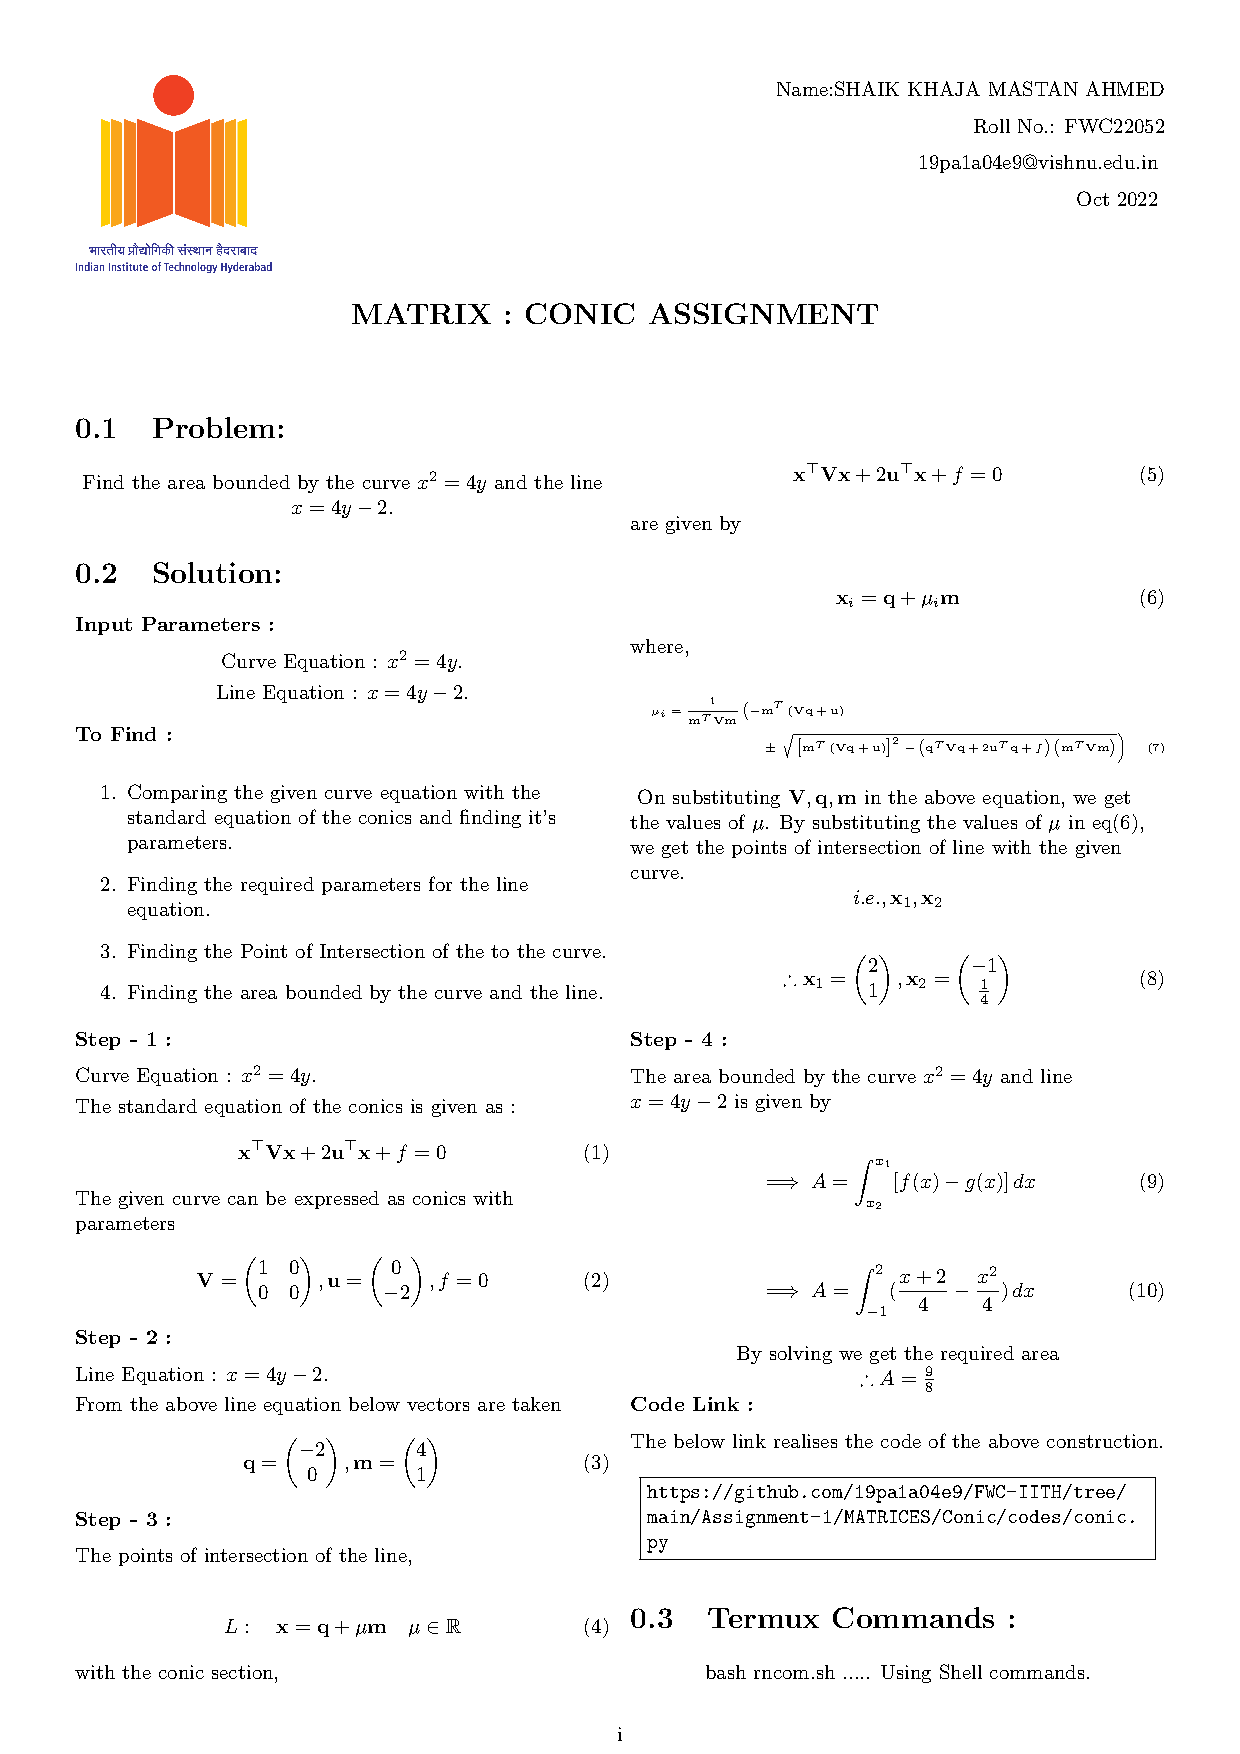
\includegraphics[scale=0.6]{../../../python/figs/conic.pdf} 
 \end{center}\vspace{1mm}
 
 \vspace{2mm} \textbf{Construction}
\begin{center}
\setlength{\arrayrulewidth}{0.5mm}
\setlength{\tabcolsep}{6pt}
\renewcommand{\arraystretch}{1.5}
    \begin{tabular}{|l|c|}
    \hline 
    \textbf{vertex} & \textbf{coordinates} \\ \hline
  $\vec{q}$ & $\myvec{
   at^2\\
   2at
   } $\\\hline
      \end{tabular}
  \end{center}
  
\raggedright  Download the code \\
Github link: \href{https://github.com/KrishnaYadati/Assignments/blob/main/Matrix_conic_assignment/codes/conic.py}{Assignment-6}.
  \end{multicols}
\end{document}
\fi
